\documentclass[UTF8]{article}

\usepackage{CTEX}
\usepackage{epstopdf}
\usepackage{amsmath}
\usepackage{amsfonts}
\usepackage{amssymb}
\usepackage{multirow}
\usepackage{adjustbox}
\usepackage{float}
\usepackage{graphicx}
\usepackage{subcaption}

\begin{CJK}{UTF8}{song}
\title{基于加速度传感器的双人体感乒乓球游戏\\
数字逻辑设计实验报告}
\author{计44~~王子云~~2014010303\\
计44~~柯云劼~~2014012086
}
\end{CJK}
\date{ }

\begin{document}
\maketitle
\newpage
\tableofcontents
\newpage
\section{实验简介}
% 柯
体感游戏是视觉与本体和动作控制的集合,为了达到视觉与运动相结合的目的,采用加速度传感器与VGA显示器相结合的方法,通过JY901传感器的运动来完成对游戏界面中的拍的控制,双方博弈模拟真实的乒乓球游戏。实验实现了开始界面、计分、自动难度调解与游戏结束等功能,最后通过下载验证,游戏获得了较好的互动性、参与性与沉浸感。
\section{总体设计思路}
% 王
我们将整个项目划分成了8大主要模块:顶层模块、SRAM控制模块、键盘控制模块、游戏控制模块、VGA模块、游戏逻辑模块、物理逻辑模块、传感器控制模块。
\begin{figure}[H]
  \centering
  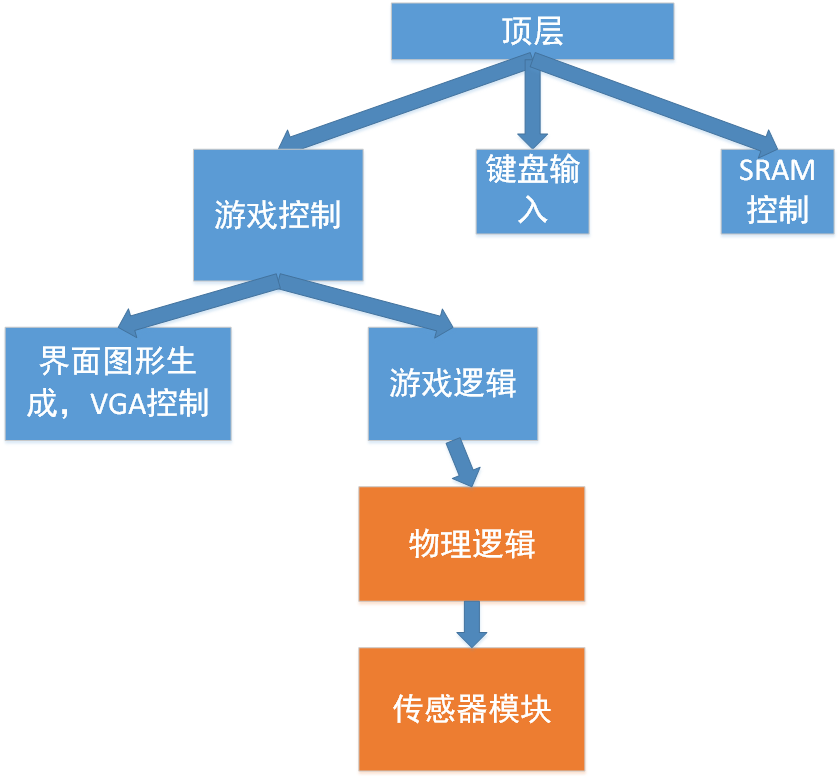
\includegraphics[width=10cm]{1-1.png}
  \caption{模块概要设计图}
\end{figure}
模块间的相互关系见上图。各个模块具体的功能如下:
\begin{itemize}
  \item 顶层模块:整个设计的最顶层,负责与外界的通信,将各个信号分别传给需要的模块。
  \item SRAM控制模块:按时序关系从SRAM中读数据,并封装好交给游戏控制模块。
  \item 键盘控制模块:处理PS2接口读到的键盘数据,解析ENTER和ESC键,封装成一个vector交给游戏控制模块。
  \item 游戏控制模块:游戏控制部分的顶层模块,负责解析外部的键盘信息,将操作分别传给VGA和逻辑,并且负责将每一时刻逻辑给出的游戏状态传给VGA。
  \item VGA模块:负责所有和VGA有关的内容,包括计算待显示的内容,计算当前像素所需图片对应的SRAM地址,处理行场同步信号。
  \item 游戏逻辑模块:这个模块处理有关游戏规则的部分,主要是记录分数。
  \item 物理逻辑模块:这个模块根据拍的位置、力度计算拍与小球的碰撞,得到球每一时刻的角度和速度,并据此计算每一时刻小球的位置。
  \item 传感器控制模块:解析传感器传来的串口信息、给出球拍的位置和检测到的挥拍力度(水平方向上的加速度)。
\end{itemize}

\section{关键技术分析}
% 自己写自己的
\subsection{加速度传感器模块}
使用uart串口协议,一根数据输出线接入TX,一根数据读取线接入RX。
	\begin{figure}[H]
		\centering
		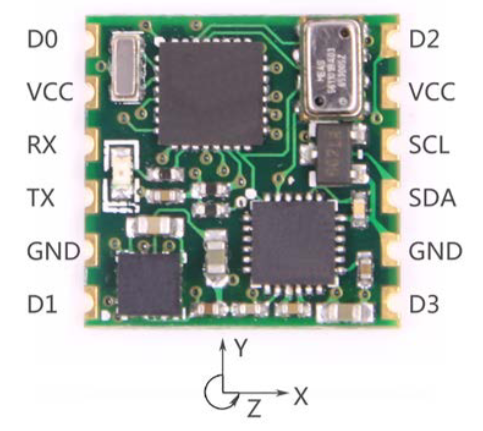
\includegraphics[width=2in]{2-1.png}
			\caption{JY901加速度传感器}	
	\end{figure}
\subsubsection{uart协议解析}
双方约定好时钟信号频率,波特率:115200(所以不像i2c或spi协议需要时钟线,但也造成了双方时钟可能会出现些偏差,导致会出现部分丢包现象)\par
获取由01电平组成的8字节长的数据包,双方统一约定电平拉低为8字节数据开始,电平拉高为8字节数据结束。\par
\subsubsection{传感器数据解析}
其中核心数据由16进制发送,也就是两个数据包组合为一个完整数据。默认第一个为低电平,第二个为高电平,需要将二者组合成一个有符号的short类型的数据。\par
多个数据组合为一个完整的输出,其中首项为设备地址,次项为输出地址,末项为校验和。\par
输出的具体解析公式方式如下:
	\begin{figure}[H]
		\centering
		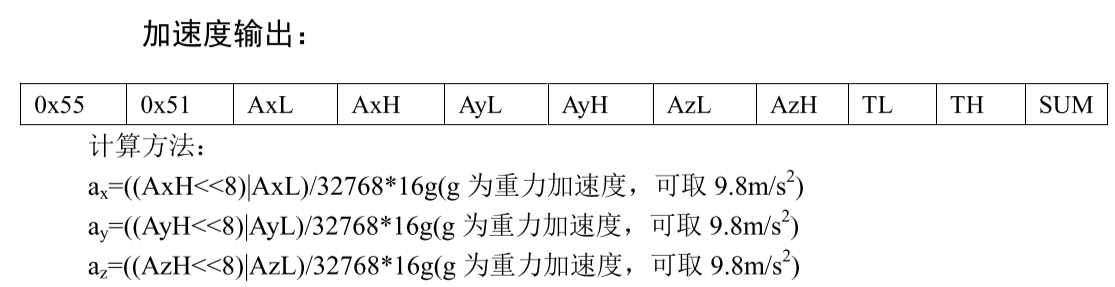
\includegraphics[width=\linewidth]{2-2.png}
			\caption{JY901加速度输出}	
	\end{figure}
	\begin{figure}[H]
		\centering
		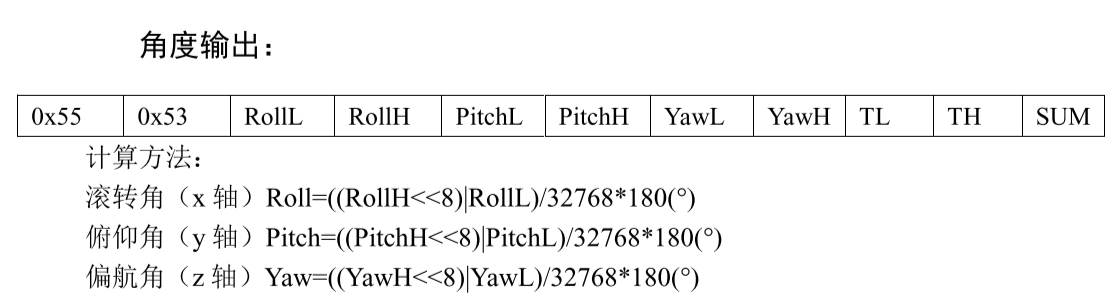
\includegraphics[width=\linewidth]{2-3.png}
			\caption{JY901姿态角输出}	
	\end{figure}

\subsection{VGA控制模块}
游戏场景的最终显示示意图如下:
\begin{figure}
  \centering
  \begin{subfigure}{.5\textwidth}
  \centering
  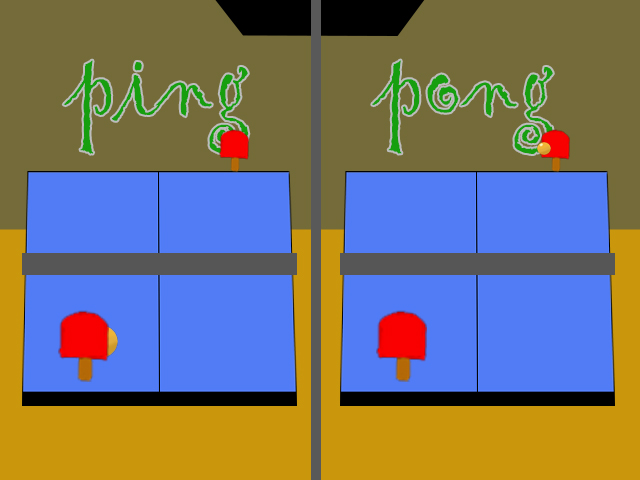
\includegraphics[width=6cm]{2-9a.jpg}
  \caption{ }
  \end{subfigure}%
  \begin{subfigure}{.5\textwidth}
  \centering
  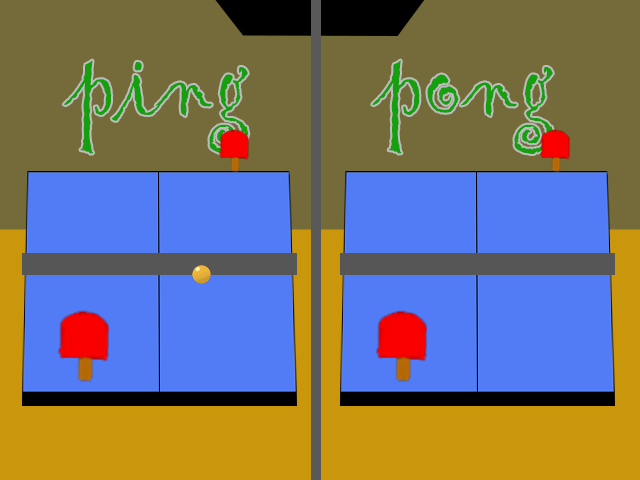
\includegraphics[width=6cm]{2-9b.jpg}
  \caption{ }
\end{subfigure}
\caption{游戏场景图}
\label{fig:game}
\end{figure}
\subsubsection{3D效果}
为了使游戏参与者有更真实的体验,我们将画面做成了类3D的视角。为了便于说明,我们采用如下的方式建立坐标系:
\begin{figure}[H]
  \centering
  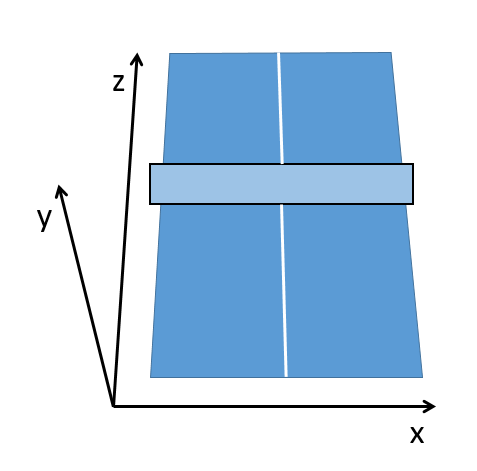
\includegraphics[width=6cm]{2-10.png}
  \caption{世界坐标系}
\end{figure}
将3D场景投影到2D的屏幕上,需要遵循基本的透视原理,因此我们的球和球拍都需要根据位置的$z$分量进行缩放,在屏幕上的竖直位置也与其$z$轴位置有关(为了减小计算量,我们近似地认为屏幕上水平方向的位置与$z$无关)。于是我们提出以下的变换关系(以左边屏幕为例):
\[\begin{aligned}
x_s&=k_{x0} + k_{x1} * x / X\_MAX \\
y_s&=k_{y0} + k_{y1} * (Y\_MAX - y) / Y\_MAX + k_{y2} * (Z\_MAX - z) \\
r&=k_{r0} + k_{r1} * (Z\_MAX - z)
\end{aligned}\]
其中,$x_s$、$y_s$分别表示在屏幕上的水平、竖直中心位置,$r$表示其边长的一半。因此,该元素(球或球拍)在屏幕上的位置是从$(x_{s}-r, y_{s}-r)$到$(x_{s}+r,y_{s}+r$的正方形。

为了节约储存空间,我们利用同一张资源图,根据$r$,利用待显示图与原图的相似关系进行缩放。若当前扫描到的点在正方形内,则有
\[\begin{cases}
    x' = x_{screen} - (x_s-r) / (2 * r) * A \\
    y' = y_{screen} - (y_s-r) / (2 * r) * A
  \end{cases}\]
其中$x_{screen}$、$y_{screen}$表示屏幕上当前扫描到的点的位置,$x'$、$y'$表示素材图上对应的坐标,$A$为素材图的边长。

\subsubsection{遮挡关系}
从示意图\ref{fig:game}上来看,不同的物体之间存在着遮挡关系:如左图中球拍会挡住一部分球、球会挡住对面的一部分球拍;右图中球在中间时可能会被中间的挡板挡住。此外,当球与球拍跑出屏幕区域,例如跨过中间竖直的分界线时也不能被显示。

为了正确地显示一系列遮挡关系,我分了球拍1、球、球拍2、背景四个图层,先将所有图层都读进来,默认为‘000000000’。为了显示球和球拍周围一圈的透明效果,我在资源文件中将要透明的地方颜色也设为‘000000000’。故如果此时读到(除背景外)某个图层颜色为全0,那么就直接不显示这一图层。按图层顺序,再配合一系列复杂的逻辑判断,就可以正确地显示场景信息。

由于球和球拍的素材图较小,它们都直接存放在片内ROM中,而背景图片存放在SRAM中。
\begin{figure}[H]
  \centering
  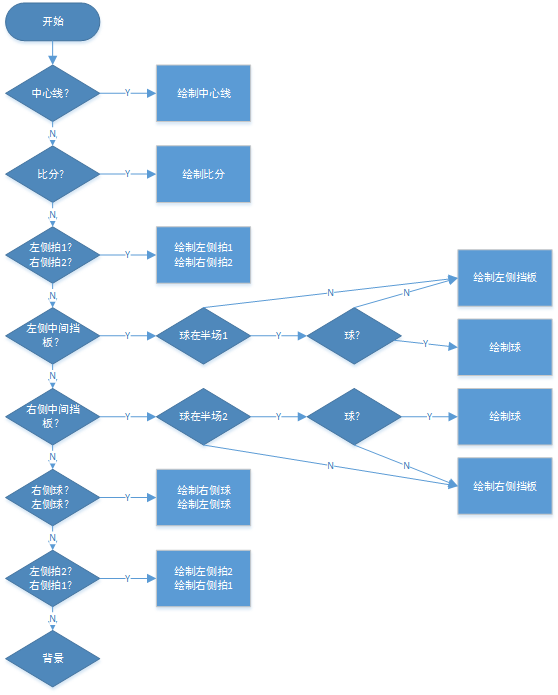
\includegraphics[width=10cm]{2-11.png}
  \caption{显示游戏场景的流程图}
\end{figure}

\section{下载验证及演示说明}
% 柯
\subsection{游戏中传感器操作方法}
初始预先设定将传感器片水平,将x轴方向指向前侧,y轴方向指向右侧。
\begin{enumerate}
\item 挥拍操作:传感器快速向前方击出
\item 移动拍操作:传感器绕x轴左右转动
\end{enumerate}
\subsection{游戏流程说明}
\begin{enumerate}
\item 游戏烧入至FPGA板上后,VGA显示器上显示开始界面。
\item 按RST建重置使游戏进入准备状态
\item 按键盘Enter,从开始界面进入游戏状态
\item 游戏预设先由屏幕左方发球。
\item 发球时球在与拍面夹角为$60^\circ-120^\circ$的区间内在拍面前来回转动。
\item 击出球后,球按着之前的轨迹在三维空间内运动。考虑到传感器操作比起实际运动的差异,故为了提供较好的用户体验,这里设置在左右边界处会发生碰撞使得游戏不会过早终止。
\item 当球进入另一方的击球区域后,若对方在球前方作出击球动作,则球被击回,挥拍力度将作为球的速度,进入6。
\item 若无法及时作出击球回应,则当球过了己方边界己方判负,对方获得一分,同时由对方发球,进入5。
\item 最先获得7分的一方获得本轮胜利,进入结束画面。
\item 按ESC可开始新一轮游戏,进入4。
\end{enumerate}
\section{实验中遇到的问题}
\subsection{传感器输出到游戏的物理运算}
\subsubsection{关于传感器的坐标变换}
之前设计中打算采用加速度进行二次积分出位置的方法:\par
传感器给出的加速度是以体轴坐标系作为参考的,\par
	\begin{figure}[H]
		\centering
		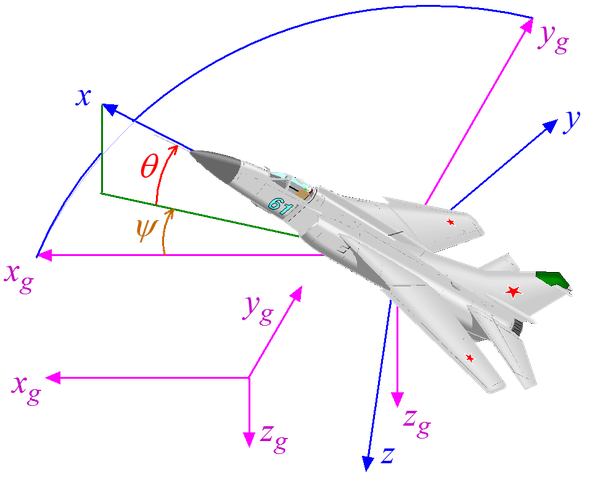
\includegraphics[width=3in]{2-4.png}
			\caption{体轴坐标系}	
	\end{figure}
故数据为了使用需要乘以一个体轴坐标系到地轴坐标系的变换矩阵。
这里介绍地轴坐标系到体轴坐标的变换,而所求变换即是原变换的逆操作。
原变换以先绕x轴旋转,再绕y轴旋转,最后绕z轴旋转进行。
	\begin{figure}[H]
		\centering
		
\includegraphics[width=3.5in]{2-5.png}
	\end{figure}
	\begin{figure}[H]
		\centering
		
\includegraphics[width=3.5in]{2-6.png}
	\end{figure}
	\begin{figure}[H]
		\centering
		
\includegraphics[width=3.5in]{2-7.png}
	\end{figure}
	\begin{figure}[H]
		\centering
		
\includegraphics[width=\linewidth]{2-8.png}
			\caption{地轴坐标系到体轴坐标的变换矩阵}	
	\end{figure}
注意到该变换矩阵是正交矩阵,所求逆矩阵即为该矩阵的转置。
\subsection{三角函数的获得}
由于三角函数是浮点值,而FPGA中不支持浮点运算,考虑乘以1000来表示原三角函数值,在运算末尾再除以1000即可。\par
又由于FPGA没有简单的获得三角函数值得方法,经取舍后决定使用rom来读取。

\subsection{SRAM相关}
当很早发现背景图片不能存在片内ROM中时,就开始考虑用SRAM存储。然而一开始并不知道如何从外部写入SRAM,也不知道应该用什么格式写入。那时与周围的同学交流,大家都还没有搞出来,于是只能主要靠自己摸索,也从老师那里得到了很多宝贵的意见,最后逐渐知道了应该用实验室的电脑上的RLab,向SRAM写入二进制文件。

搞定了外部写入的问题之后,又发现屏幕上显示的画面与预期严重不符。在老师的建议下,我学会了用SignalTap进行调试,搞清楚了原来是自己制作二进制文件时,高位到低位的顺序写反了。

\subsection{显示的位置不匹配}
从之前的示意图可以看到,我们将屏幕分成了两边,对应于双方不同的视角。对同一个对象(如球),要根据一个三维坐标分别计算两侧不同的二维显示位置,而且要显得协调、真实,确实不是一件容易的事情。我临时改用键盘控制球在空间中移动,观察屏幕上的显示,然后慢慢调整参数,最终找到一个合适的参数使得看起来有3D的感觉,而不会觉得特别奇怪。

\section{总结与体会}
% 王
一开始我们提出这个游戏的想法的时候,是希望能做一个和真实的乒乓球一样的游戏,可以将传感器绑在乒乓球拍上,通过挥拍来进行游戏。后来发现传感器的控制比我们想象的要困难许多,要想做到在传感器任意角度下准确地计算出世界坐标系中的加速度、速度、位移太困难,误差太大。于是我们不得不放低要求,考虑怎么样才能在“可以实现”的前提下尽可能地有趣。于是我们修改了游戏规则,让球可以碰到墙壁反弹;我们简化了物理运算,同时又考虑了挥拍的力度击球的角度,让球速和方向可以变化,增强竞技性和趣味性。

虽然过程中遇到了很多挫折,遇到了很多意想不到的困难, 投入了大量的时间,在实验室奋战到深夜过,也担心过到底能不能按时完成。但是最后,在演示的前一天晚上,我们终于把各种bug解决掉,可以握着两只传感器,痛痛快快地对打一场的时候,我们感受到了无比的成就感。这次大作业也让我们看到了其他同学的创造力,各个组的作品都非常厉害。记得展示之前几天,我们逐渐看到各个组的项目一点点趋向完成,大家彼此参观、试玩,真的十分有趣。

最后,我们想感谢在整个项目过程中帮助过我们的老师、助教和同学们。感谢老师每周和我们交流,让我们一直有进展,并且遇到问题随时可以请教;感谢助教的辛勤付出,尤其是展示的前夜陪我们各组成员奋战到深夜;感谢其他小组的同学们毫不吝啬地互相帮助,传授彼此会的技能。感谢这门课提供这样的机会,让我们磨炼了硬件编程的技能,也体会到了用硬件编程的挑战与乐趣。

\end{document} 